\chapter{Conclusion}
\label{chap:conclusion}

This dissertation presents a motion planning approach suited for
multi-step manipulations tasks.
Key to the approach are the complementary ideas of \emph{lazy}
and \emph{utility-guided} search,
which we integrated into the LEMUR motion planning algorithm.
This approach has shown promising results on manipulation tasks
when compared with state-of-the-art
search-based and sampling-based anytime planners.
This concluding chapter begins by summarizing the dissertation
and the individual algorithmic contributions
in Section~\ref{sec:conclusion:summary}.
This is followed by a discussion in Section~\ref{sec:conclusion:future}
of a few promising avenues for future research
which build on our results.
Finally, we offer some concluding remarks
in Section~\ref{sec:conclusion:remarks}.


\section{Summary and Contributions}
\label{sec:conclusion:summary}

This dissertation focuses on motion planning problems
which arise in autonomous manipulation tasks.
Such tasks induce continuous, high dimensional robot configuration
spaces
in which path validity checking is particularly expensive
due to complex robot kinematics and workspacee geometry.
Furthermore,
there is an inherent cost tradeoff between
planning a motion and subsequently executing it.
For manipulation tasks in human-scale environments in particular,
whether measured in time or energy,
the cost of planning (principally path validity checking)
is comparable to the cost of execution.
Therefore,
reasoning over both sources of cost -- and their tradeoff --
is paramount.

To address these challenging motion planning problems,
this dissertation proposes a collection of algorithms
(Figure~\ref{fig:conclusion:outline})
which work in concert to minimize both planning and execution cost.
We first motivate our focus on roadmap methods for motion
planning,
and then consider two central questions concerning the search
over those roadmaps:
(a) how should we conduct the optimization,
and (b) what objective should we optimize?

\begin{figure}[t]
   \centering
   \includegraphics{build/outline}
   \caption{Outline of the algorithms developed in this dissertation.
      LEMUR is solves a continuous motion planning problem via
      discretization as a series of progressively densified roadmaps
      (Chapter~\ref{chap:roadmaps}).
      Since the shortest path problem over the resulting graph
      in characterized by edge costs which are expensive to evaluate,
      we exploit lazy search and edge selectors
      (Chapter~\ref{chap:lazysp}) to minimize planning effort.
      We also develop a novel incremental bidirectional search
      algorithm (Chapter~\ref{chap:ibid}) to accommodate the resulting
      dynamic pathfinding problem.
      LEMUR conducts its search guided by a utility function
      (Chapter~\ref{chap:utility}) which can employ distinct
      domain-specific planning and execution cost heuristics.
      In multi-step manipulation tasks,
      one such cost model is derived from the family motion planning
      problem (Chapter~\ref{chap:family}),
      which leads to planner invocations which minimize combined
      planning and execution cost.
      }
   \label{fig:conclusion:outline}
\end{figure}

\subsection{Motion Planning via Roadmaps}

In Chapter~\ref{chap:roadmaps},
we outlined the motion planning problem,
as well as a selection of algorithms designed to solve it.
A wide variety of such algorithms exist,
including optimization-based, search-based, and sampling-based
planners.
We motivate our focus on sampling-based roadmap planners
based on the following advantages:
\begin{itemize}
\item Roadmap methods are well-studied and posess favorable
   theoretical properties such as asymptotic optimality.
\item It is straightforward to incrementally densify the
   discretization by adding new samples to the roadmap.
\item The cost of constructing a roadmap which is
   insensitive to the distribution of obstacles can be amortized
   across all planning queries
   (e.g. loaded from disk and persisted in memory between queries).
\end{itemize}

The algorithms presented in this dissertation are agnostic to the
particular roadmap structure used for the discretization.
Our experiments were conducted over roadmaps generated
via Halton sequences,
with edges between vertices within a connection radius
determined by the critical value $\gamma^*_{\mathcal{C}}$.
For example, the LEMUR motion planner
(Algorithm~\ref{alg:lemur} in Chapter~\ref{chap:utility})
densifies its roadmap by introducing new batches of
vertices and edges;
in our experiments,
we reduce the connection radius as recommended in
\citep{janson2015deterministicsampling}.
We discuss future avenues for treating roadmaps
in Section~\ref{subsec:conclusion:future-roadmaps}.

\subsection{How to Optimize?}
Committing to a particular discretization (e.g. roadmaps)
reduces the continuous motion planning problem
to a discrete graph pathfinding problem.
The first central question considered in this dissertation, then,
is how a motion planning objective should be optimized over
such a roadmap graph.

\paragraph{Lazy Pathfinding.}
Pathfinding for motion planning problems is distinguished from other
shortest-path applications because
the primary component in its edge objective
depends on its \emph{validity},
which expensive to determine for articulated robots.
This motivates lazy pathfinding approaches,
which decouple the search for candidate solutions
from the process of evaluating each solution for its cost.

The first contribution of this dissertation is a study of
the LazySP algorithm outline in Chapter~\ref{chap:lazysp},
\marginnote{Contribution: The LazySP algorithm,
which exploits an edge selector to find paths while
minimizing the number of necessary edge weight evaluations.}
which allows for this edge evaluation to be specified arbitrarily
by way of an \emph{edge selector} function.
We show that simple selectors are equivalent to the existing
Weighted A* and Lazy Weighted A* pathfinding algorithms,
and we also consider the efficacy of bidirectional
and bisection selectors.

We then introduce novel selectors based on path distributions,
which focus evaluations towards edges which most likely lie on
a shortest path.
One such path distribution selector is based on the partition
function over paths on a graph.
\marginnote{Contribution: an incremental method to maintain
the partition function over paths under changing edge weights.}
We develop an incremental method for 
We show that these selectors can lead to fewer expected edge
evaluations than their simple alternatives over a set of example
problems.
We also motivate why the alternating strategy serves as
a simple proxy for the more complex path distribution selectors
for common cases where no a priori knowledge of the obstacle
distribution exists.

\paragraph{Dynamic Pathfinding.}
Conducting our roadmap search over candidate paths via lazy
pathfinding
induces an underlying inner dynamic shortest path problem.
This arises because the decoupled nature of lazy search
is indistiguishable from a search over an unknown or changing objective.
Each iteration of our lazy search constitutes a new dynamic planning
episode --
after our edge selector nominates particular edges of our roadmap
for evaluation and their true costs are determined,
the inner search must accommodate these changes in order to produce
new candidate paths on subsequent iterations.

Existing incremental algorithms for dynamic pathfinding problems,
such as Lifelong Planning A* \citep{koenig2004lpastar},
make use of heuristic potential functions to reduce the subset of
the graph that must be considered when solving each planning episode.
During a lazy search,
the strength of this heuristic depends on
the relationship between the true and estimated edge weights
($w$ and $w_{\ms{est}}$ in LazySP, respectively)
-- and in many cases, a strong lower bound on $w$,
and therefore a strong heuristic, may not exist.
This motivates our study of the dynamic problem
in Chapter~\ref{chap:ibid}.

A common approach to solving pathfinding problems in domains without
a strong heuristic is the notion of bidirectional search.
Unifying bidirectional and incremental methods presents a unique
challenge,
since the subtle bidirectional termination condition must be
posed in such a way that it remains applicable even under the
changing edge weights which arise in a dynamic problem.
This allows us to formulate the Incremental Bidirectional Dijkstra's
(IBiD) algorithm,
\marginnote{Contribution: the IBiD algorithm,
an incremental and bidirectional shortest path algorithm
for dynamic graphs.}
which generalizes the bidirectional Dijkstra's algorithm
\citep{goldberg2005spexternalmemory}
in the same way that the DynamicSWSF-FP algorithm
\citep{ramalingam1996dynamicswsffp} generalizes the original
Dijkstra's algorithm \citep{dijkstra1959anote}.
We also show how this algorithm can be adapted in the presence of
heuristic potential functions.
This algorithm shows promising results both on road network routing
problems (Chapter~\ref{chap:ibid})
as well as inflated lazy search problems from motion planning.

\subsection{What to Optimize?}
Our treatment of lazy roadmap search deliberatively leaves open
the question of what objective should be optimized.
The approach is applicable to any pathfinding domain in which
the edge weight function $w$ is expensive to evaluate,
and where an inexpensive estimate $w_{\ms{est}}$ may be available.
In the case of motion planning for articulated robots,
where planning and execution cost are both important,
how should we instantiate these functions?

\paragraph{Search over Candidate Utility.}
In Chapter~\ref{chap:utility},
we introduce the notion of \emph{utility},
and argue that it is the correct form of the objective in order
to capture the tradeoff between planning and execution costs.
Our conception of utility borrows heavily from the BUGSY algorithm
\citep{burns2013bugsy} for conventional graph search.
The key insight is that marrying utility with lazy search
allows for the incorporation of planning cost estimators over
concrete candidate paths -- and not just over frontier vertices.
This enables many domain-specific planning heuristics to be
represented naturally.

We next show that by committing to
(a) a utility function that is linear in planning and execution cost,
and (b) estimators that are additive over path edges,
we can represent our utility optimization as a lazy shortest path
problem.
Mediated by the tradeoff parameter $\lambda_p$,
the LEMUR algorithm
\marginnote{Contribution: the LEMUR motion planning algorithm
which conducts a lazy search guided by path utility over a set of
sequence of densified roadmaps.}
conducts this optimization
over a sequence of progressively densified roadmaps.

We examine a set of manipulation planning tasks using three
robot platforms,
and conduct experiments using a planning cost heuristic which
captures the remaining collision checks on each candidate path.
We show that LEMUR exhibits favorable performance
when compared against a set of anytime planners
such as RRT-Connect, BIT*, and Lazy ARA*.

\paragraph{Utility Estimates in Manipulation Planning.}
Importantly,
the utility-based objective described in Chapter~\ref{chap:utility}
allows arbitrary domain-specific planning cost estimates
to be leveraged.
Chapter~\ref{chap:family} explores intelligent heuristics
in manipulation tasks by formulating such multi-step tasks as
a \emph{family motion planning problem}.
\marginnote{Contribution:
the family motion planning problem
a formulation of manipulation planning that yields a natural
planning cost estimate for utility-guided motion planners.}
We show this representation,
in which multi-step tasks are given over a family of related
$\mathcal{C}$-space subsets,
allows for a planning cost heuristic
which naturally incentivizes a utility-based planner (such as LEMUR)
to reuse planning computation from prior queries.


\section{Future Directions}
\label{sec:conclusion:future}

Treating motion planning as a lazy search over roadmaps
prompts an array of promising directions for further work.
Improvements in roadmap discretization,
focusing of edge evaluations,
better inner search algorithms,
more expressive domain-specific planning and execution cost
heuristics,
and probabilistic optimization techniques might all improve performance
over a wide array of planning domains.
In this section,
we survey a few such promising directions that arise from our
approach.

%The remainder of this chapter discusses both the implications
%and limitations of the presented approach,
%as well as possible directions for future work.
%In this chapter,
%we discuss opportunities to extend our approach to acheive even
%better performance,
%examine options to better integrate motion planning into a
%task planning system,
%and expound on other promising future directions.

\subsection{Improved Roadmaps}
\label{subsec:conclusion:future-roadmaps}

One of the fundamental questions in any motion planning approach
is how should the continuous problem be approximated in order
to search for a solution.
The approach to motion planning presented in this dissertation
relies fundamentally on the roadmap discretization method.
The approach can therefore benefit from any technique which improves
the efficacy of this discretization.

\paragraph{Better Connection Heuristics.}
Roadmap methods rely on a connection rule to determine whether
two vertices representing configurations in the $\mathcal{C}$-space
should be connected with an edge
-- the existance of such an edge implies that the local planner
has high likelihood of successfully finding a valid path between them.
To this end,
most approaches make use of arbitrary thresholds of
simple distance functions over $\mathcal{C}$ as their decision rules.
In our experiments, for example,
we used a simple Euclidean distance rule.

However, for articulated robots
(and especially for recurring tasks in similar environments),
it is easy to conceived of more intelligent connection rules.
For example, consider a na\"{\i}ve execution cost model in which
obstacles are distributed unformly in the robot's workspace.
In this case,
the likelihood of collision over some edge length
depends intimately on the configuration of the arm itself
-- configurations in which the Jacobian matrix is large
(where changes in the location of robot geometry are large
with respect to changes in configuration)
entail higher collision probability.
In the case of recurring motion planning queries for the same
robot geometry,
it would seem beneficial to pre-compute a roadmap structure
in which the edge connection rule depends on some similar measure
of the robot's configuration.

\paragraph{Efficient Densification.}
Smarter sequences that are easy to densify.
Fractal patterns?
Not lattices.
Parallelization.
Recent RSS results?

\subsection{Adaptive Roadmap Densification via an Infinite Roadmap Stack}
\label{sec:discussion:disc}
The LEMUR planner effectively conducts its search over a sequence of
progressively densified roadmaps
(Figure~\ref{fig:discussion:roadmap-stack}).
The results presented in this thesis have used Halton sequences
as discussed in Chapter~\ref{chap:roadmaps}
for their prefereable dispersion properties,
and form a roadmap graph using an $r$-disk connection rule.
As discussed in \citep{janson2015deterministicsampling},
the shorest path on such a sequence of roadmaps
posesses asymptotic optimality if the connection radius is adjusted
appropriately.

\begin{figure}
   \centering
   \includegraphics{build/roadmap-stack}
   \caption{A stack of progressively densified roadmaps
      over a given free configuration space $\mathcal{C}$.}
   \label{fig:discussion:roadmap-stack}
\end{figure}

\paragraph{Hard batching.}
Like many existing roadmap-based algorithms
\citep{starek2015bfmtstar, gammell2015bitstar},
LEMUR implements a hard batching approach to densification --
a search is conducted fully over each batch of the roadmap
in $\mathcal{C}$
until a solution is found.
While the specification of LEMUR allows for this roadmap to be
implicitly constructed,
the current implementation constructs the entire batch before
proceeding with its search.
Once the search over that roadmap completes without a feasible path found,
the next batch of vertices and edges are added to the graph,
and the newly densified roadmap is searched.

Because the sequence of roadmaps that is searched is insensitive to
the distribution of obstacles,
the current implementation of LEMUR is able to pre-compute a sequence
of roadmaps up to a certain level of discretization,
and then load that roadmap structure into memory directly
instead of building it from scratch for each planning query.

There are two shortcomings that arise from this hard batching approach:

\begin{itemize}
\item \emph{Uniform Densification:}
   The fact that this roadmap is loaded uniformly across the space
   is certainly a limitation that will become restrictive
   in spaces of larger dimension.
\item \emph{Densification vs. Resolution Completeness:}
   The current LEMUR algorithm only moves to a denser roadmap
   once no finite paths are shown to be available on the present
   roadmap.
   This may not be desirable in large spaces --
   it may make sense to move to a denser roadmap in the vicinity of
   a short path before exploring all corners of the space.
\end{itemize}

There are a number of promising avenues for a solution
to the problems that arise from uniform densification..
Informed anytime algorithms
\citep{gammell2014informedrrtstar, gammell2015bitstar}
restrict densification once an initial path is found to a subset of
the full space that may contain better solutions.
This approach is not directly applicable
because LEMUR is not an anytime algorithm.

\paragraph{Adaptive Roadmap Densification.}
An alternative strategy is to adopt an adaptive densification approach
under which the search is conducted upon an infinite stack of
progressively densified roadmaps.

Consider the roadmap stack depicted
in Figure~\ref{fig:discussion:roadmap-stack-onramps}.
Here, as before,
each underlying roadmap is a superset of the one above it.
But now,
instead of progressively considering each layer individually
(using batching),
consider conductiong a single search over the entire stack.
Note that the stack includes additional edges
(shown dotted in the figure)
connecting corresponding vertices in two adjacent layers;
using a road network analogy,
we call these edges ``offramp'' edges.
A proposed edge weighting scheme involves two components:
(a) an artificial inflation of edge weights by some factor
on each layer according to a schedule
(with edges on lower layers inflated more),
and (b) an artificial constant weight assigned to each offramp edge
between layers.

%Related to the idea of adaptive dimensionality
%\citep{gochevetal2011adaptivedim}
%(large portions of solutions can be low-dimensional).

\begin{marginfigure}
   \centering
   \includegraphics{build/roadmap-stack-onramps}
   \caption{A roadmap stack with ``offramp'' edges.}
   \label{fig:discussion:roadmap-stack-onramps}
\end{marginfigure}

Consider a search over this infinite stack $G$
between two start and destination
configurations corresponding to distinguished vertices on $G$,
and consider an optimal solution path with strong $\delta$-clearance.
If the roadmap layers satsify the appropriate conditions
(e.g. connection radius
\citep{karaman2011samplingoptimal, janson2015deterministicsampling}),
and all roadmap edges have non-negative weight,
and all ``offramp'' edges have some constant positive weight $\alpha$,
then we conjecture that there exists a shortest path $p$ through $G$
of finite length (which traverses a finite number of layers of $G$).
Furthermore,
we conjecture that the length of $p$ approaches the length of an
optimal path as $\alpha \rightarrow 0$.

We find this representation of the continuous problem compelling
because it natually integrates the densification problem with
the search problem.
One can imagine a unidirectional or bidirectional search
effectively trading off between
exploring more widely on a particular layer
and descendng to a denser layer in order to traverse a narrow passage.
Descending to a denser layer occurs natually during the search,
and denser regions can be sampled on demand only in areas of the space
adjacent to obstacles blocking the path.
Furthermore,
the computational cost of such densification can be captured as
an additional planning cost component in the LEMUR algorithm,
so it will commit to a denser layer only when the predicted path
savings outweigh the requisite planning cost.

\subsection{Improved Lazy and Dynamic Search}

The core of our approach is a lazy search over candidate paths,
which makes use of an inner dynamic shortest path problem
in order to select candidates at each iteration.
There are a number of potential avenues available for making this
search more efficient.

\paragraph{Intelligent Selection of Key Edges.}
In Chapter~\ref{chap:lazysp},
we presented novel edge selectors which maintain a distribution over
candidate paths
in order to focus edge evaluations towards edges which most likely
lie on a short path.
While this showed promising results across a range of problem instances,
maintaining this distribution can incur its own computational cost
(quadratic in the number of vertices in the case of the Partition
selector),
and therefore it can be intractable over large roadmap graphs.

The effect of these selectors is to automatically discover
and focus on the parts of the motion planning problem that are
most constrained.
It would be worthwhile to explore ways of more efficiently maintaining
such path distributions for larger graphs.
In the case of a bidirectional evaluation strategy
(such as the Alternate selector),
it may be beneficial to attempt to discover online which end
of the problem proves to be the most constrained.

It may also be instructive to investigate the ``oracle'' selector.
Consider that for any graph,
there exists some minimal set of edges which, if evaluated,
would proveably demonstrate that the best remaining candidate is
correct.
Investigating the distribution of edges required for such a selector
for particular problem instances
may aid in desigining new selectors.
It also serves as a useful benchmark against which to compare performance.

\paragraph{Exploring the Interaction between Lazy and Dynamic Search}
Lazy search induces an inner dynamic shortest path problem,
as edge weights are updated and intermediate candidate paths are
required.
When LEMUR addresses a problem with $\lambda_p > 0$,
so that planning cost is to be considered in its utility objective,
it generally selects candidates that do not solely minimize execution cost
in favor of candidates that lower remaining planning cost.

Paradoxically,
as the $\lambda_p$ parameter is increased,
the underlying dynamic search problem becomes more difficult,
because its heuristic is no longer as strong.
(A consistent heuristic typically only exists for the component of
the edge weight function derived from the execution cost component.)
It would therefore be beneficial to investigate schemes whereby
the requirement for optimal shortest paths from the inner
dynamic search is relaxed.
For example,
consider a variant of the LazySP algorithm
in which the candidate path at each iteration only maximizes utility
up to a particular suboptimality bound. 
One suitable algorithm for this relaxed dynamic serach problem
is Truncated Incremental Search \citep{aine2016truncatedincremental}.

\paragraph{Adjusting the Incremental Balancing Criterion.}
It is well-known \citep{pohl1969bidirectional}
that using the cardinality of each OPEN list as the decision rule
to balance expansion of the two sides of a bidirectional search
generally outerforms using the distance (key) value itself.
Unfortunately,
it is not clear how to adapty this criterion to the incremental
search setting,
since the size of the queue of inconsistent vertices is no longer
indicative of the density of the graph on the two sides.
Can we dynamically adjust the distance balance criterion
so that the location of the interface between the two trees
(represented as the edge connection queue)
approximates this balanced cardinality criterion?

\subsection{Better Planning Cost Estimates}

The planning cost model we used for our experiments in this thesis
was very simple:
each collision check entails a constant amount of computational cost.
There are a number of ways that our model can be improved:
\begin{itemize}
\item The planning cost incurred by performing a collision check
   can be estimated dynamically,
   either across a planning episode,
   or as a function of the check's location in the C-space.
\item We can include planning cost models for additional aspects of
   the planner which can be costly.
   Two immediate candidates are
   (a) the cost of conducting an additional inner search
   over the lazy graph,
   and (b) the cost of progressing to a denser roadmap graph.
   Accommodating these estimates may lead to a more natural
   termination condition as well.
\end{itemize}

\subsection{Maximizing Utility in Expectation}

Progressive densification is a proxy for handling the
spatial coherence in the scene.
What if we handle this more explicitly?

The LEMUR algorithm exploints an optimistic assumption when considering
candidate paths for prospective evaluation:
it assumes all unevaluated edges are collision-free.
While this assumption allows the inner loop to process candidates
quickly,
it requires the hard batching approach to strike an artificial
balance between local and global exploration.
It is worth investigating whether abandoning the optimistic
assumption is worthwhile --
a replacement would reason explicitly about the collision probability
across the configuation space.

We recently proposed a first step in this direction
via the Pareto Optimal Motion Planner \citep{choudhury2016pomp}.
In this work,
we maintain a probabilistic model of the probability of collision
across the configuration space,
which we update incrementally as collision checks are performed
agains the environment.
The planner then uses this model in order to select candidate paths
for partial evaluation that minimize some combination of the path's
execution cost and its probability of collision.



%\cdnote{Talk about Shushman's POMP stuff.}
%
%The purpose of the incremental graph densification strategy
%achieved by hard batching (Chapter~\ref{chap:utility})
%is to account for spatial correlation
%in $\mathcal{C}_{\mbox{\scriptsize free}}$.
%We would like to motivate this more formally.
%
%We propose to extend the E$^8$-PRM planner
%to minimize ensemble effort \emph{in expection}
%using a probabalistic model of $\mathcal{C}_{\mbox{\scriptsize free}}$.
%Even if this is too expensive,
%we can motivate the incremental densification idea,
%with a graduated cost model
%to approximate a probabalistic model
%of the $\mathcal{C}$-space.
%
%How should discrete graphs be constructed in continuous
%   $\mathcal{C}$-spaces with spatially correlated execution costs?
%
%Chapter~\ref{chap:graphs-in-continuous}
%discusses how to embed roadmaps in $\mathcal{C}$
%so that they can be searched by E$^8$.
%
%The problem with na\"{\i}vly running E$^8$ on a
%dense roadmap in $\mathcal{C}$
%is that it tends to bunch up in local minima.
%This is because reducing the continuous planning problem
%to a graph search ignores the spatial correlation
%inherent in $\mathcal{C}_{\mbox{\scriptsize free}}$.
%
%One way to capture this is to maintain a probabalistic model
%of $\mathcal{C}_{\mbox{\scriptsize free}}$,
%and then optimize in expectation.
%In particular,
%instead of greedily choosing the best path based on
%optimistic estimates of one-time planning and execution cost:
%\begin{equation}
%   f(\pi) = \lambda \hat{f}_p(\pi) + (1-\lambda) \hat{f}_x(\pi),
%\end{equation}
%we instead reason over the total \emph{expected} remaining cost:
%\begin{align}
%   f(\pi)
%      &= E \left[ \lambda f_p(\pi) + (1-\lambda) f_x(\pi) \right] \\
%   &= P_{\mbox{\scriptsize free}}(\pi)
%      \left[ \lambda \hat{f}_p(\pi) + (1-\lambda) \hat{f}_x(\pi) \right]
%      + (1-P_{\mbox{\scriptsize free}}(\pi))
%      \left[ \lambda F_p + (1-\lambda) F_x \right]
%\end{align}
%
%Consider the the problem from Figure~\ref{fig:example-in-expectation}.
%There are an infinite number of paths to the goal,
%each consisting of walking along the sidewalk,
%followed by crossing the street perpendicuarly at a particular
%position $x$.
%The sidewalk is known to be collision-free,
%whereas each position on the street must be tested for collision
%with obstacles with planning validation cost $\hat{f}_p(\pi)$
%independent of $x$.
%Execution cost $f_x(\pi)$ is given by $|x|+c$.
%
%Suppose we first test walking straight across the street $\pi_0$
%(knowing nothing, this is clearly the optimistically cheapest path)
%and this is deemed in collision.
%Which path should we consider next (e.g $\pi_a$ or $\pi_b$)?
%
%What is our model for $P_{\mbox{\scriptsize free}}(\pi)$?
%Relate to GPs for classification\cite{rasmussen2006gpml}.
%
%We are operating under assumptions:
%\begin{itemize}
%\item Single-shot greedy (won't choose \emph{sets} of paths
%   which minimize remaining effort)
%\item Operates over \emph{paths} instead of configurations
%   or edges (won't probe points, no explicit exploration)
%\end{itemize}
%
%\begin{figure}
%   \begin{center}
%   \includegraphics{build/example-in-expectation}
%   \end{center}
%   \caption{Simple example problem to illustrate optimizing
%      remaining ensemble cost in expectation.}
%   \label{fig:example-in-expectation}
%\end{figure}

\subsection{Integration with Collision Checking}

Most sampling-based planners consider the collision checker
to be a block box;
given a configuration $q_{\ms{test}}$,
this procedure considers the environment
and the robot's kinematics,
and returns a boolean answer -- True or False.
Depending on the fidelity of the geoemtric model of the robot
and environment,
each check can entail tens, hundreds, or even thousands
of microseconds;
precious planning time which can detract from the robot's overall
task performance.

One avenue for minimizing the computation effort spent performing
collision checks is integrate directly with the broad-phase
algorithm which effectively identifies configurations for which
many (or all) geometric pairs are sufficiently far from collision
that the more expensive narrow-phase checks need not be applied.

\begin{figure}
   \centering

   % left side
   \subfloat[Paths with lambda=0][%
      \centering
      Paths with $\lambda = 0$\par
      Average length: 733.0\par
      Average check cost: 7219.5
   ]{
      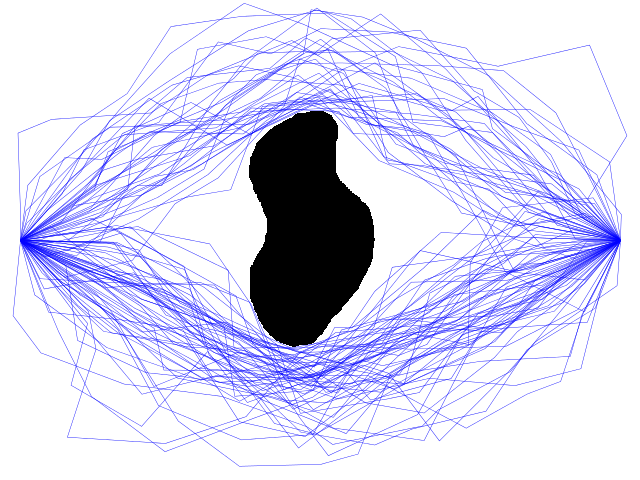
\includegraphics[width=0.45\textwidth]
      {figs/bean-allpaths-lambda0.png}
   }
   % right side
   \subfloat[Paths with lambda=1][%
      \centering
      Paths with $\lambda = 1$\par
      Average length: 836.5\par
      Average check cost: 4692.6
   ]{
      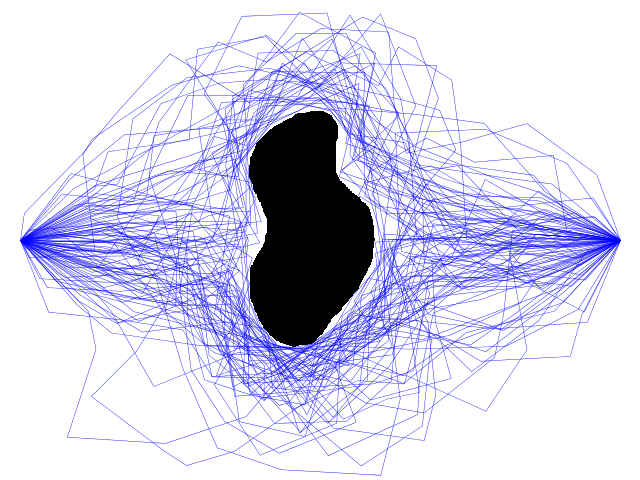
\includegraphics[width=0.45\textwidth]
      {figs/bean-allpaths-lambda1.png}
   }
   \\
   \subfloat[Paths with lambda=0][%
      \centering
      Paths with $\lambda = 0$\par
      Average length: 733.0\par
      Average check cost: 2685.7
   ]{
      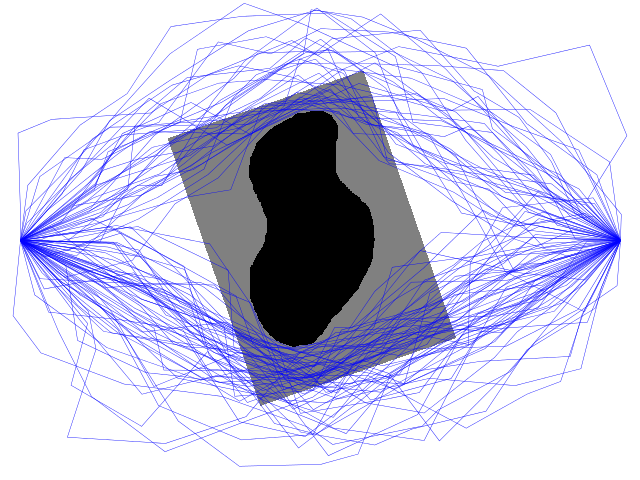
\includegraphics[width=0.45\textwidth]
      {figs/bean-allpaths-padded-lambda0.png}
   }
   % right side
   \subfloat[Paths with lambda=1][%
      \centering
      Paths with $\lambda = 1$\par
      Average length: 907.1\par
      Average check cost: 1064.5
   ]{
      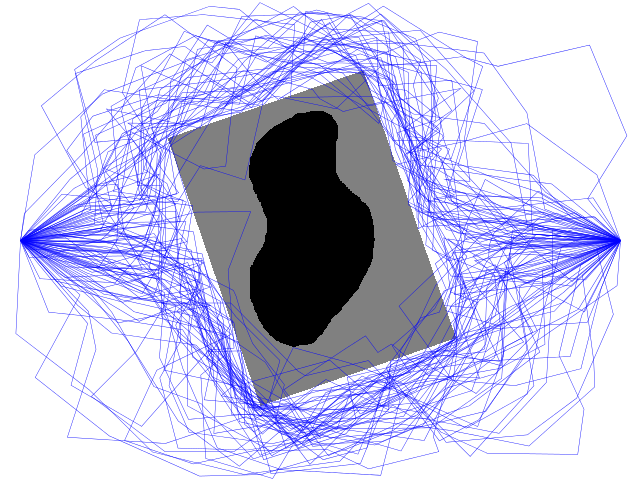
\includegraphics[width=0.45\textwidth]
      {figs/bean-allpaths-padded-lambda1.png}
   }

   \caption{A simple 2D example of the Multi-Set PRM using
     a broad-phase check.
     Checking for collision with the grey box is 10x less expensive
     than with the actual black obstacle.}
     %\cdnote{I need to talk about this in the text.}}
   \label{fig:broad-phase-2d}
\end{figure}

\begin{figure*}
   \centering
   
   \subfloat[
      A motion planner testing simply for membership in
      $\mathcal{C}_{\mbox{\scriptsize free}}$
      treats a collision validity checker as a
      ``black box.''
      Internally,
      modern checkers first employ an inexpensive broad-phase check
      using a low-dimensional conservative representation
      to quickly identify non-colliding bodies before
      resorting to an expensive narrow-phase check.
   ]{%
      \includegraphics{build/broadphase-single}%
   }%
   \quad%
   \subfloat[
      A family motion planner can explicitly reason about the
      conservative nature of the broad-phase check.
      This allows it to defer some narrow phase checks
      (often indefinitely)
      and instead prefer paths that require fewer expensive checks.
   ]{%
      \includegraphics{build/broadphase-multi}%
   }
   
   \caption[][0.0in]{Collision validity checking is a commonly used
     indicator function.
     The family motion planning formulation allows an intelligent
     planner to reach inside the checker's ``black box''
     and reduce the number of costly narrow-phase checks.
     Resulting paths tend to be cheaper to compute and
     stay further from obstacles.}
   \label{fig:broad-phase}
\end{figure*}

Consider the illustrative motion planning example shown
in Figure~\ref{fig:broad-phase-2d},
and the corresponding two-phase system described
in Figure~\ref{fig:broad-phase}.

\cdnote{
More caching!
Hypothesized volumes / Cell decompositions.
Bored robots.
Similarity to Leven/Hutchenson.
}

\subsection{Tighter Motion Planner Integration in a Planning System}

A motion planner is one component in a larger planning system for
an articulated robot performing real-world tasks.
There are opportunities for improved system performance by
integrating the planner more tightly with other system components.

\subsection{Integration with stuff above}

ISER task planning.
Cite ISER paper.

Task and motion planning.

I did some work on CMR stuff for multi-step problems,
for instance.
Cite this.

\paragraph{Task and Motion Planning.}
Other recent work has married symbolic reasoning with geometric planning
for tasks with multiple subtasks
as multi-modal planning \citep{hauser2010multi},
temporal logic \citep{bhatia2010temporalgoals},
or hierarchical or bridged representations and interfaces
\citep{cambon2009hybrid}, \citep{gravot2005asymov},
\citep{srivastava2014taskmotion}.

Treat an entire multi-step plan using LazySP (each edge is expensive after all!)

\paragraph{Other Applications of LazySP.}
\cdnote{Talk about satellite application from that guy.}

\section{Concluding Remarks}
\label{sec:conclusion:remarks}

Here are some concluding remarks.

Lazy and utility-guided are complementary.

Lazy effectively decouples planning from evaluation.
Accomplishes the same thing as BIT* ellipsoid.
